This chapter uses definitions adapted from \cite{van2013process, hompes2015detecting, baier2015matching} to give a background of the formalization of event logs, Petri nets and alignments. First off, some basic mathematical foundations are required.

\begin{definition}[Tuples]
For sets $X_1, X_2, \ldots, X_n$, $t \in X_1 \times X_2 \times \ldots \times X_n$ is an $n$-tuple. For $1\le i\le n$, $t_i$ is the projection on the $i$th element in the tuple.
\end{definition}

\begin{definition}[Functions]
For sets $X$ and $Y$, $f:X\to Y$ is a total function and $g: X\nrightarrow Y$ is a partial function. The domain of a function is the set of elements it is defined on, so $dom(f) = X$ and $dom(g) \subseteq X$ because a partial function does not have to be defined on every element. All elements in the domain are mapped to an element in the target set $Y$.
\end{definition}

\begin{definition}[Powerset]
For a set $X$, $\mathcal{P}(X)=\set{S}{S \subseteq X}$ denotes the set of all subsets of $X$.
\end{definition}

\begin{definition}[Multiset]
For a set $X$, a multiset $B:X\to \mathbb{N}_0$ over $X$ is a set with duplicates. $B(x)$ gives the frequency of $x$ in $B$. Multisets use square brackets e.g. $B_1=[a,a,b,c,c,c,c]=[a^2,b,c^4], B_2=[a,d]$. They overload the typical set operations $B_1 \uplus B_2 = [a^3,b,c^4,d], B_1 \cap B_2 = [a]$ and $B_1 \setminus B_2 = [a,b,c^4]$. The set of all multisets over $X$ is $\mathcal{B}(X)$.
\end{definition}

\begin{definition}[Sequences]
For any set $X$, $\sigma = \langle \sigma_1, \sigma_2, \ldots, \sigma_n \rangle \in X^*$ is a finite sequence over $X$ of length $|\sigma|=n$. $set(\sigma) = \set{x\in X}{\exists 1 \le i \le |\sigma|: \sigma_i = x}$ is the set of distinct elements in the sequence $\sigma$.
Two sequences $\sigma, \sigma^\prime \in X^*$ can be concatenated to $\sigma \cdot \sigma^\prime$, e.g. $\langle a,b \rangle \cdot \langle c \rangle = \langle a, b, c \rangle$.
Any (partial) function $f:X \nrightarrow Y$ to some set $Y$ can be applied to a sequence over $X$ recursively as follows. $f(\langle \rangle) = \langle \rangle$ and for $x\in X$ and $\sigma \in X^*$: 
$$f(\langle x \rangle \cdot \sigma) = \begin{cases}
f(\sigma) & \text{if } x\notin dom(f)\\
\langle f(x) \rangle \cdot f(\sigma) & \text{if } x \in dom(f)
\end{cases}$$
A sequence over $X$ can also be projected onto a subset $Q\subseteq X$ recursively. So $\langle \rangle \restriction_Q = \langle \rangle$ and for $x\in X$ and $\sigma \in X^*$: $$(\langle x \rangle \cdot \sigma)\restriction_Q = \begin{cases}
\sigma\restriction_Q & \text{if } x\notin Q\\
\langle x \rangle \cdot \sigma\restriction_Q & \text{if } x \in Q
\end{cases}$$
Sequences over tuples $\sigma \in (X_1 \times \ldots \times X_m)^*$ can be projected to a sequence over $X_i$ ($1\le i\le m$) with $\sigma \restriction_i$.
\end{definition}

\begin{definition}[Logic]
For a set $X$ and a formula $\phi:X\to \mathcal{B}$, $\forall x\in X: \phi(x)$ requires $\phi$ to hold for all $x$, $\exists x\in X: \phi(x)$ requires $\phi$ to hold for at least one $x$ and $\exists!\ x\in X : \phi(x)$ requires $\phi$ to hold for exactly one $x$. For two formulas $\phi$ and $\psi$, $\phi \wedge \psi$ requires both to hold, $\phi \vee \psi$ requires at least one to hold and $\phi \XOR \psi$ requires exactly one of them to hold.
\end{definition}

The recording of events during process execution is the basis of all process mining activities. Recorded events are always associated with an activity and a time. Other attributes are optional.
\begin{definition}[Event]
Let $\E$ denote the universe of all possible events. The set $ATE$ contains all possible event attribute names. For an event $e \in \mathcal{E}$ and attribute name $n\in ATE$, $n(e)$ is the value of attribute $n$ of event $e$. If $e$ does not have attribute $n$, $n(e)=\bot$. $\Univ A$ denotes the universe of all activities. The event attributes $activity:\mathcal{E}\to \Univ A$ and $time: \E \to Time$ are always defined.
\end{definition}
For readability, we write events together with their activity in the superscript like $e^{activity(e)}$.
Traces are a chronologically ordered sequence of such events and belong to a case along with possible further case attributes. Since events are considered to be unique, there cannot be any duplicates in a trace.
\begin{definition}[Trace]
A trace $\sigma = \langle e_1, e_2, \ldots, e_n \rangle \in \mathcal{E}^*$ is a finite sequence of events without duplicates, i.e. $\forall 1\le i < j\le n: e_i \neq e_j$. The events are non-strictly ordered by their time attribute, i.e. $\forall 1\le i < j\le n: time(e_i) \le time(e_j) $.
\end{definition}
Like an event, a case is a unique object with attributes, one of which being the associated trace.
\begin{definition}[Case]
Let $\C$ denote the universe of all possible cases. The set $ATT$ contains all possible case attribute names. For a case $c\in \C$ and attribute name $n \in ATT$, $n(c)$ is the value of attribute $n$. If $c$ does not have attribute $n$, $n(c) = \bot$. The attribute $trace(c)=\hat{c}\in \mathcal{E}^*$ is always defined. $\hat{c}$ will be used as a shorthand for the associated trace of a case.
\end{definition}
An event log is a collection of cases.
\begin{definition}[Event log]
Let $\Log \subseteq \C$. $\Log$ is an event log if every event in the log is unique, i.e. $\forall c,c^\prime \in \Log: c\neq c^\prime \implies set(\hat{c}) \cap set(\hat{c}^\prime) = \emptyset$. The universe of event logs is $\Univ L$.
\end{definition}

As a notation for process models, we use (labeled) Petri nets. Observe that, since different process notations (like BPMN models) can be converted between each other, this is not a restriction.
\begin{definition}[Labeled Petri net]
A (labeled) Petri net is a tuple $PN=(P,T,F,l)$ consisting of the set of places $P$, set of transitions $T$ with $P \cap T = \emptyset$, a flow relation $F\subseteq (P \times T) \cup (T \times P)$ and a labeling function $l:T \to \Univ A \cup \{ \tau \}$, with $\tau \notin \Univ A$. The labeling function maps each visible transition to an activity in $\Univ A$. Transitions $t\in T$ mapped to $\tau$ are called silent or invisible. They are unobservable. The sets $T^l=\set{t\in T}{l(t)\neq \tau}$ and $T^{\tau}=\set{t\in T}{l(t)=\tau}$ partition the transitions into those labeled with an activity and the silent ones.
\end{definition}
To be able to refer to adjacent nodes more easily, the preset and postset are defined. For places they contain transitions and for transitions places.
\begin{definition}[Preset, postset]
Let $PN=(P,T,F,l)$ be a Petri net. For every node $n\in P \cup T$, $n^\bullet=\{m | (n, m) \in F\}$ is the postset and $^{\bullet}n=\{m | (m, n) \in F\}$ the preset of $n$.
\end{definition}
A marking describes the state of a Petri net, represented by a distribution of tokens on the places.
\begin{definition}[Marking]
Let $PN=(P,T,F,l)$ be a Petri net. A marking $M\in \mathcal{B}(P)$ is a multiset of places. For every $p\in P$, $M(p)$ is the number of tokens on place $p$. A transition $t\in T$ is enabled in a marking $M$, written $M[t \rangle$, if each place in $\pre t$ has at least one token. The transition execution $M[t \rangle M^\prime$ results in the marking $M^\prime = (M \setminus \pre t) \uplus \post t$ where one token is removed from every place in the preset and one is added to every place in the postset.
\end{definition}
To make a Petri net executable, an initial marking which describes the initial distribution of tokens and a final marking which describes a valid completion states are required.
\begin{definition}[System net]
A system net $SN=(PN,M_i,M_f)$ is a Petri net $PN=(P,T,F,l)$ with an initial marking $M_i$ and final marking $M_f$. A valid firing sequence on $SN$ is a sequence of transitions $\sigma \in T^*$ such that $\forall 1\le j \le |\sigma| : M_{j-1}[\sigma_j \rangle M_{j}$ with $M_0=M_i$ and $M_{|\sigma|}=M_f$ where every transition execution was enabled.
\end{definition}

\begin{figure}
    \centering
    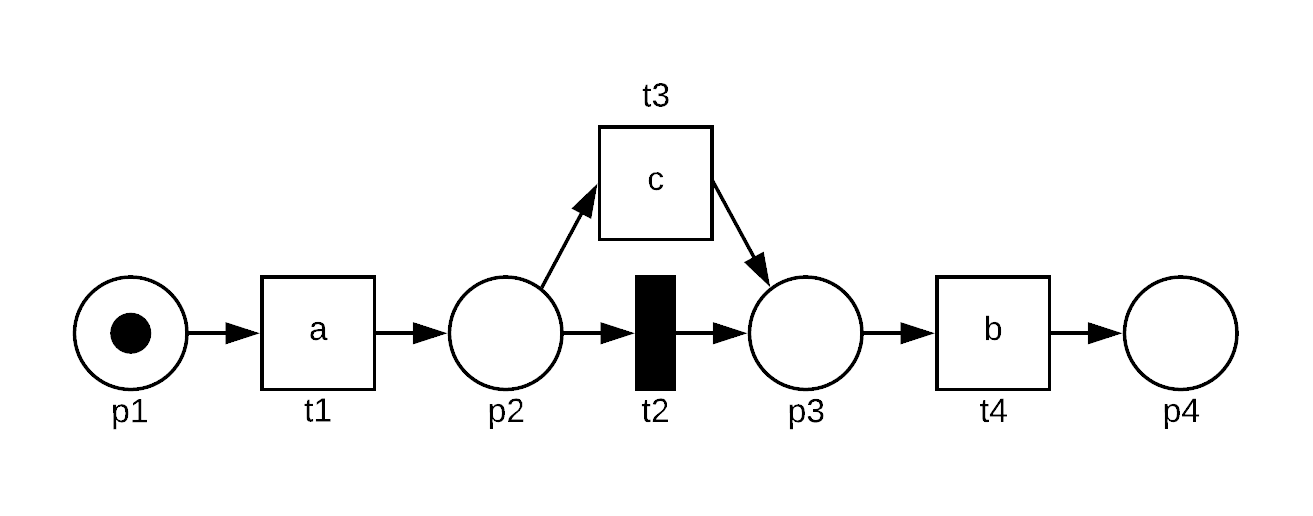
\includegraphics[width=.6\textwidth]{figures/preliminaries/simplenet.png}
    \caption{A simple Petri net}
    \label{fig:simplenet}
\end{figure}

\begin{figure}
    \centering
    $\gamma_1=\bigalignment{4}{$e_{11}$ & $e_{12}$ & $e_{13}$ & \doublegg}{b & a & c & }{\doublegg & a & c & b}{ & t1 & t3 & t4}$ and $\gamma_2=\bigalignment{3}{$e_{21}$ & \doublegg & $e_{22}$}{a & & b}{a & $\tau$ & b}{t1 & t2 & t4}$
    \caption{Two example alignments for $\hat{c}_1 = \langle e_{11}^b, e_{12}^a, e_{13}^c \rangle$ and $\hat{c}_2 = \langle e_{21}^a, e_{22}^b \rangle$}
    \label{fig:simplealign}
\end{figure}
For replaying a (possibly unfitting) trace on a system net which might contain silent transitions or multiple transitions with the same label (duplicate transitions) alignments from \cite{van2012replaying} are being used.
\begin{definition}[Alignment]
Let $SN=(PN, M_i, M_f)$ be a system net and $c\in \C$ a case. An alignment $\gamma \in (\E \cup \{\gg\}) \times(T \cup \{ \gg \}) \setminus \{(\gg,\gg)\}$ is a sequence of so-called moves such that $\gamma\restriction_1\restriction_{\E} = \hat c$ and $\gamma\restriction_2\restriction_T$ is a valid firing sequence on $SN$. And for every $1\le i \le |\gamma|$:
\begin{itemize}
    \item $\gamma_i = (e,t)$ with $e\in \E$, $t\in T$ is called a move in both and if $activity(e) = l(t)$ it is called a synchronous move,
    \item $\gamma_i = (e,\gg)$ with $e\in \E$ is called a log move,
    \item $\gamma_i = (\gg, t)$ with $t\in T$ is called a model move and if $l(t) = \tau$ it is called an invisible move.
\end{itemize}
Since there may be multiple valid alignments, a cost function is used to rank them and return the optimal one. The standard cost function, which is often used, gives sync moves and invisible moves cost $0$ and move on model/log cost $1$. A move on both which is not a synchronous move gets a cost of $\infty$ since it is usually not wanted. For the cost of the whole alignment, the costs for all moves are summed up.
\end{definition}
Figure \ref{fig:simplealign} shows two example alignments for the traces $\hat{c}_1 = \langle e_{11}^b, e_{12}^a, e_{13}^c \rangle$ and $\hat{c}_2 = \langle e_{21}^a, e_{22}^b \rangle$ on the model given in Figure \ref{fig:simplenet}. The top row contains events together with their $activity$ and the bottom row transitions together with their label to make it more readable. The alignments provide a path through the model even for unfitting traces like $\hat{c}_1$ or traces which require the execution of invisible transitions like $\hat{c}_2$.